From our trained random forest regression model, we get a glimpse of both what
useful, contributing redditors look like, and what bad, non-contributing
redditors look like.

Our test data set was about 3,200 redditors, all of their post data (around
1GB), and all of their comment data (around 3GB). From this test data set, we
used our our regressive model to get a reliability score between $-1 \leq s_r
\leq 1$. Then, we re-correlate this score with input features to intuitively see
what features are important or not, and what features indicated useful and
not-useful redditors.

\subsection{Distribution of Users} % (fold)
\label{sub:distribution_of_users}

In general, we around 24\% of users to have a negative score, and the remaining
76\% to have a positive score. This falls in line with a YouGov study that
revealed about a quarter of Americans admit to acting as `trolls', or other
sorts of argumentative, non-constructive behavior online \cite{trollstats}. A
more detailed distribution of scores is in \Cref{fig:data_20}. Most of the
scores assigned were closer to $1$, with a relatively uniform distribution of
other scores.

\begin{figure}[tb]
    \centering
    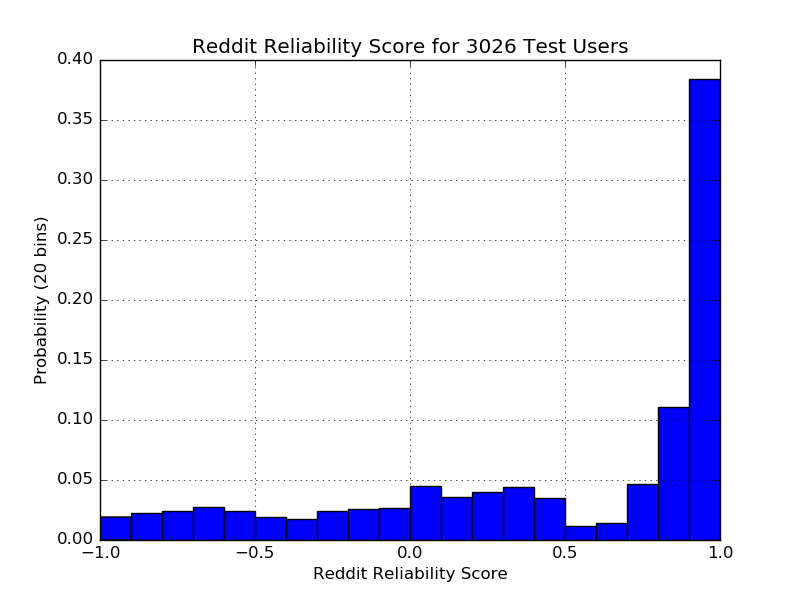
\includegraphics[width=\linewidth]{../src/do_regression/figs/data_20.png}
    \caption{The distribution of the reliability score $s_r$ of the sampled redditors, binned into twenty bins.}
    \label{fig:data_20}
\end{figure}

% subsection distribution_of_users (end)

\subsection{Feature Efficacy} % (fold)
\label{sub:feature_efficacy}

Though we gathered several different features, not all of them ended up being
`useful' in terms of creating a reliability score. The full table of the
features that we used, as well as the percentage importance our model placed on
them, appears in \Cref{tab:features}. It's worth noting that some featured are
highly correlated, like karma from top 100 subreddits and total karma, so even
though these features might be correlated with reliability, the model did not
place importance on them.

\subsubsection{What Did Work} % (fold)
\label{ssub:what_did_work}

The most important features unsurprisingly turned out to be the amount of post
and comment karma a user had. As this is the built in voting system of
\reddit{}, we expected to see this. Plots of how post and comment karma vary
with reliability appear in
\Cref{fig:reliability_post_karma,fig:reliability_comment_karma}, respectively.
Both of these plots suggest that the voting system works to root out unreliable
users; users with $s_r < 1$ don't get much karma. Of users with $s_r \geq 1$,
the distribution is bimodal. We hypothesize that our model manages to
differentiate between users who are casual, and post well received but non-
useful content, and those who post useful, reliable content which is also well
received by \reddit{} on the whole. Similarly, the voting system seems to
discourage participation from unreliable users.
\Cref{fig:reliability_post_count,fig:reliability_comment_count} suggest that
users who are unreliable do not end up posting much, but those who are more
reliable are more likely to post far more content.

A more surprising feature was the importance of a user verifying their email. A
split histogram of $s_r$ of users, split on if they have verified their email or
not (\Cref{fig:data_20_email}), suggests that though the model only placed
0.65\% importance on this feature, having an unverified email means a user is
more likely to not be reliable. This stands to reason; people who act badly on
the Internet often do so only when their anonymity is guaranteed
\cite{cho1999privacy}, as it is on \reddit{}, so they'd be less likely to link a
non-anonymous account like email to their \reddit{} account.

\begin{figure}[tb]
    \centering
    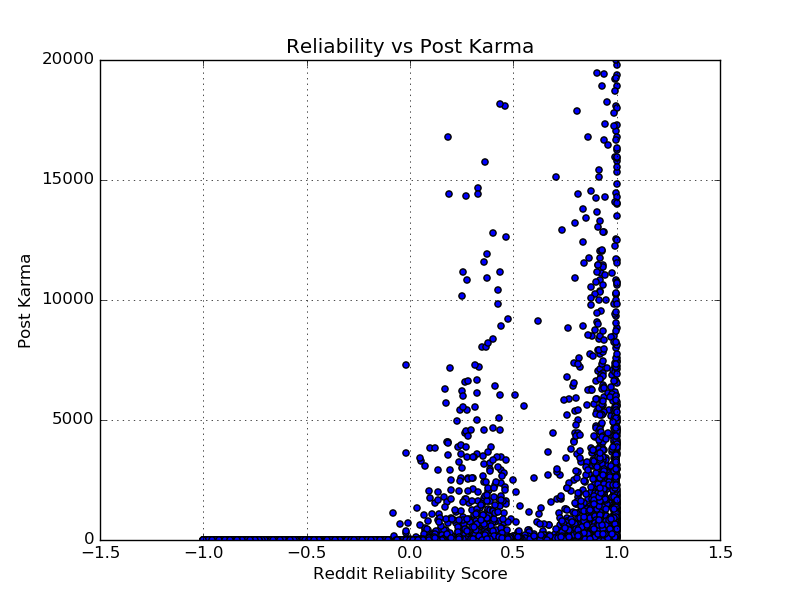
\includegraphics[width=\linewidth]{../src/do_regression/figs/reliability_post_karma.png}
    \caption{The reliability score $s_r$ plotted against the post Karma the redditor has.}
    \label{fig:reliability_post_karma}
\end{figure}

\begin{figure}[tb]
    \centering
    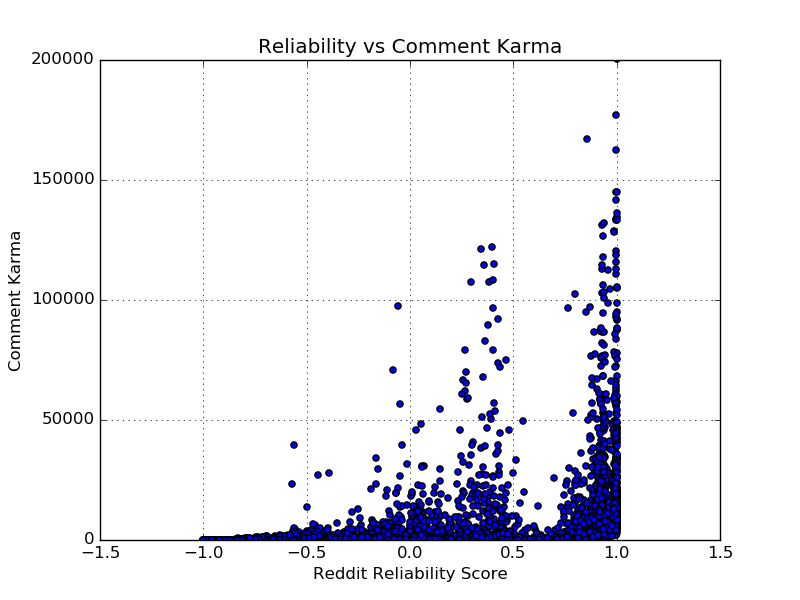
\includegraphics[width=\linewidth]{../src/do_regression/figs/reliability_comment_karma.png}
    \caption{The reliability score $s_r$ plotted against the comment Karma the redditor has.}
    \label{fig:reliability_comment_karma}
\end{figure}

\begin{figure}[tb]
    \centering
    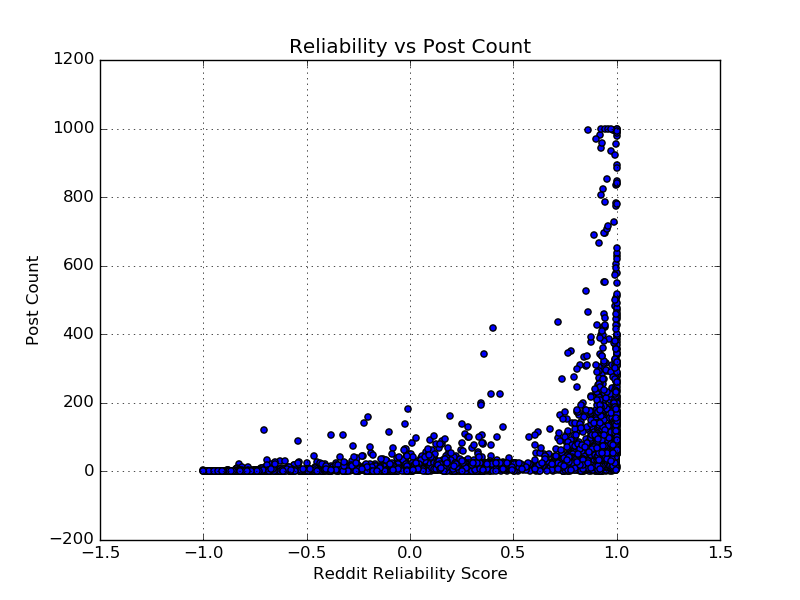
\includegraphics[width=\linewidth]{../src/do_regression/figs/reliability_post_count.png}
    \caption{The reliability score $s_r$ plotted against the number of posts the redditor has made.}
    \label{fig:reliability_post_count}
\end{figure}

\begin{figure}[tb]
    \centering
    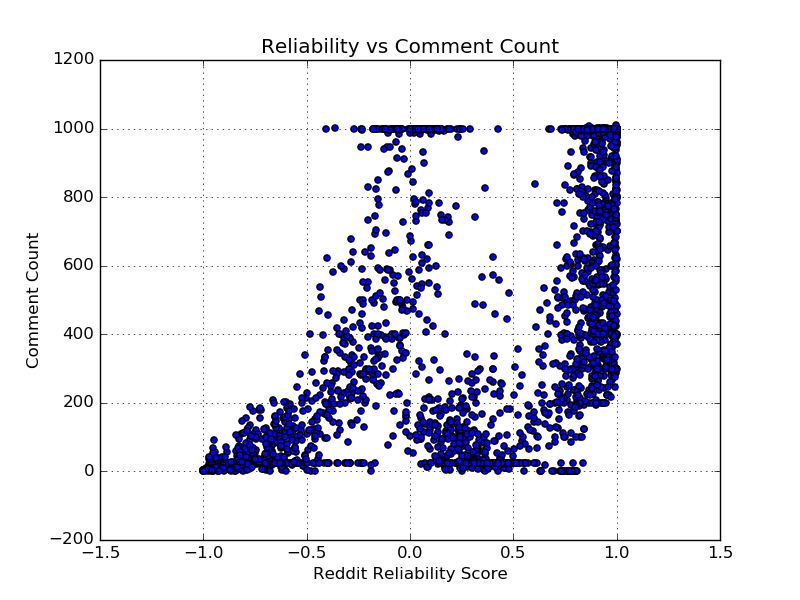
\includegraphics[width=\linewidth]{../src/do_regression/figs/reliability_comment_count.png}
    \caption{The reliability score $s_r$ plotted against the number of comments the redditor has made.}
    \label{fig:reliability_comment_count}
\end{figure}

\begin{figure}[tb]
    \centering
    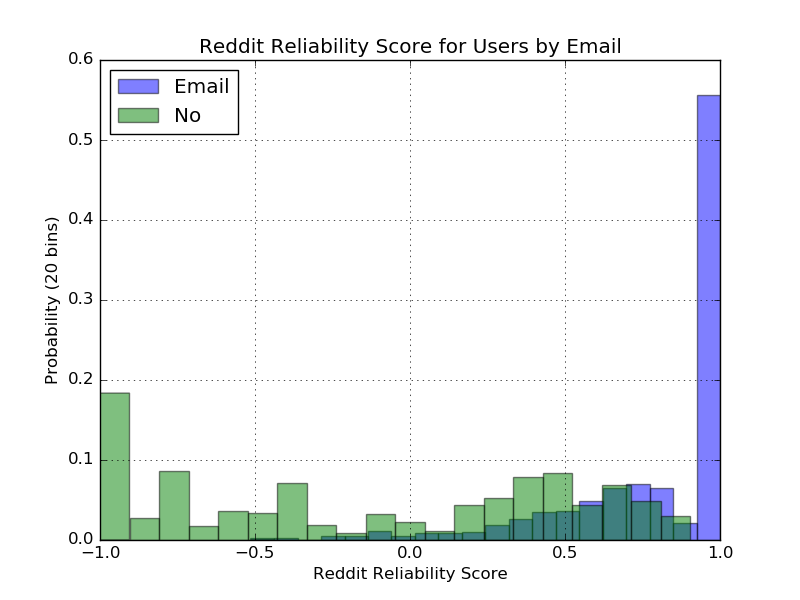
\includegraphics[width=\linewidth]{../src/do_regression/figs/data_20_email.png}
    \caption{The distribution of the reliability score $s_r$ of the sampled redditors, binned into twenty bins, separated by if they have a verified email address or not.}
    \label{fig:data_20_email}
\end{figure}

% subsubsection what_did_work (end)

\subsubsection{What Didn't Work} % (fold)
\label{ssub:what_didn_t_work}

Though we had hoped that features of the words that redditors used would
indicate how reliable they were, we didn't find this to be the case. An
examination of \Cref{fig:reliability_readability} suggest that there is not
relationship between reliability and Flesch--Kincaid readability of comments.
Our model placed similarly low importance on the frequency of using bad words
and readability of comments. This suggests to us that many kinds of speech
patterns are accepted on \reddit{}, and has little bearing on reliability. Our
model also placed low importance on the amount of karma earned in subsets of
subreddits.

We also thought that gilding would be an important feature, but it turned out
not to be, as seen in \Cref{fig:reliability_gilded}. Not enough users get gilded
on \reddit{}, which makes sense, as putting real money into the service is a
much higher friction action than simply using it for free.

\begin{figure}[tb]
    \centering
    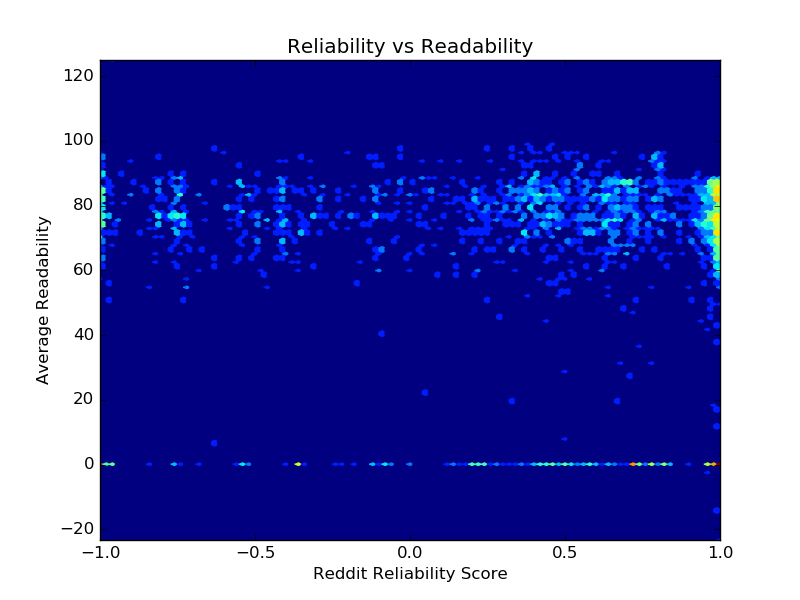
\includegraphics[width=\linewidth]{../src/do_regression/figs/reliability_readability.png}
    \caption{The reliability score $s_r$ plotted against the Flesch--Kincaid readability of their comments.}
    \label{fig:reliability_readability}
\end{figure}

\begin{figure}[tb]
    \centering
    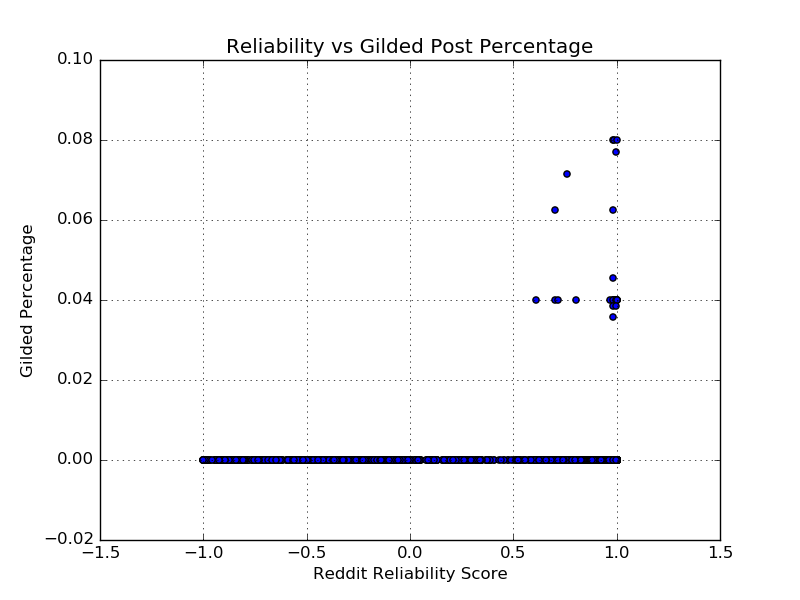
\includegraphics[width=\linewidth]{../src/do_regression/figs/reliability_gilded.png}
    \caption{The reliability score $s_r$ plotted against the percentage of gilded posts.}
    \label{fig:reliability_gilded}
\end{figure}

% subsubsection what_didn_t_work (end)

% subsection feature_efficacy (end)
